% Created by tikzDevice version 0.12.3.1 on 2021-10-13 11:14:54
% !TEX encoding = UTF-8 Unicode
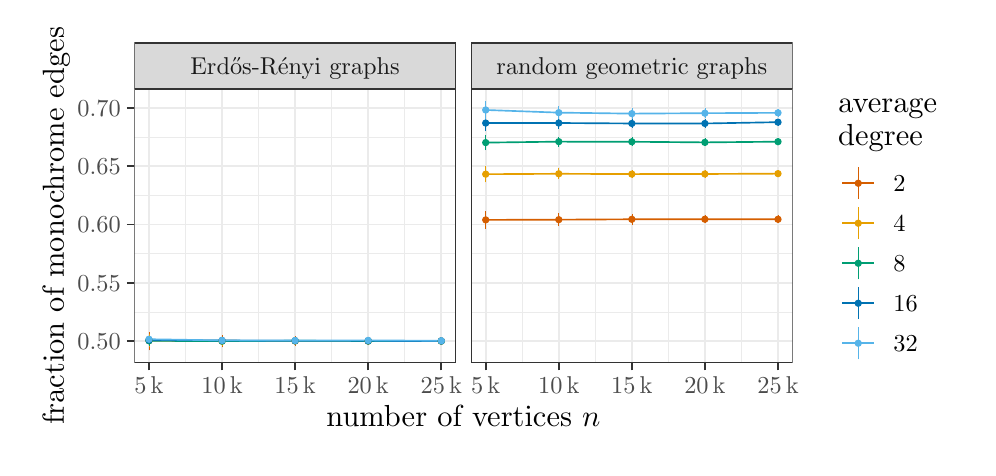
\begin{tikzpicture}[x=1pt,y=1pt]
\definecolor{fillColor}{RGB}{255,255,255}
\path[use as bounding box,fill=fillColor,fill opacity=0.00] (0,0) rectangle (339.67,151.77);
\begin{scope}
\path[clip] (  0.00,  0.00) rectangle (339.67,151.77);
\definecolor{drawColor}{RGB}{255,255,255}
\definecolor{fillColor}{RGB}{255,255,255}

\path[draw=drawColor,line width= 0.6pt,line join=round,line cap=round,fill=fillColor] (  0.00,  0.00) rectangle (339.67,151.77);
\end{scope}
\begin{scope}
\path[clip] ( 38.56, 30.69) rectangle (154.73,129.70);
\definecolor{fillColor}{RGB}{255,255,255}

\path[fill=fillColor] ( 38.56, 30.69) rectangle (154.73,129.70);
\definecolor{drawColor}{gray}{0.92}

\path[draw=drawColor,line width= 0.3pt,line join=round] ( 38.56, 49.04) --
	(154.73, 49.04);

\path[draw=drawColor,line width= 0.3pt,line join=round] ( 38.56, 70.12) --
	(154.73, 70.12);

\path[draw=drawColor,line width= 0.3pt,line join=round] ( 38.56, 91.20) --
	(154.73, 91.20);

\path[draw=drawColor,line width= 0.3pt,line join=round] ( 38.56,112.28) --
	(154.73,112.28);

\path[draw=drawColor,line width= 0.3pt,line join=round] ( 57.04, 30.69) --
	( 57.04,129.70);

\path[draw=drawColor,line width= 0.3pt,line join=round] ( 83.44, 30.69) --
	( 83.44,129.70);

\path[draw=drawColor,line width= 0.3pt,line join=round] (109.84, 30.69) --
	(109.84,129.70);

\path[draw=drawColor,line width= 0.3pt,line join=round] (136.24, 30.69) --
	(136.24,129.70);

\path[draw=drawColor,line width= 0.6pt,line join=round] ( 38.56, 38.50) --
	(154.73, 38.50);

\path[draw=drawColor,line width= 0.6pt,line join=round] ( 38.56, 59.58) --
	(154.73, 59.58);

\path[draw=drawColor,line width= 0.6pt,line join=round] ( 38.56, 80.66) --
	(154.73, 80.66);

\path[draw=drawColor,line width= 0.6pt,line join=round] ( 38.56,101.74) --
	(154.73,101.74);

\path[draw=drawColor,line width= 0.6pt,line join=round] ( 38.56,122.82) --
	(154.73,122.82);

\path[draw=drawColor,line width= 0.6pt,line join=round] ( 43.84, 30.69) --
	( 43.84,129.70);

\path[draw=drawColor,line width= 0.6pt,line join=round] ( 70.24, 30.69) --
	( 70.24,129.70);

\path[draw=drawColor,line width= 0.6pt,line join=round] ( 96.64, 30.69) --
	( 96.64,129.70);

\path[draw=drawColor,line width= 0.6pt,line join=round] (123.04, 30.69) --
	(123.04,129.70);

\path[draw=drawColor,line width= 0.6pt,line join=round] (149.45, 30.69) --
	(149.45,129.70);
\definecolor{drawColor}{RGB}{213,94,0}

\path[draw=drawColor,line width= 0.2pt,line join=round] ( 43.84, 35.19) -- ( 43.84, 41.93);

\path[draw=drawColor,line width= 0.2pt,line join=round] ( 70.24, 36.26) -- ( 70.24, 40.83);

\path[draw=drawColor,line width= 0.2pt,line join=round] ( 96.64, 36.78) -- ( 96.64, 40.36);

\path[draw=drawColor,line width= 0.2pt,line join=round] (123.04, 36.97) -- (123.04, 39.98);

\path[draw=drawColor,line width= 0.2pt,line join=round] (149.45, 37.09) -- (149.45, 40.00);
\definecolor{drawColor}{RGB}{230,159,0}

\path[draw=drawColor,line width= 0.2pt,line join=round] ( 43.84, 36.56) -- ( 43.84, 41.12);

\path[draw=drawColor,line width= 0.2pt,line join=round] ( 70.24, 36.71) -- ( 70.24, 40.13);

\path[draw=drawColor,line width= 0.2pt,line join=round] ( 96.64, 37.26) -- ( 96.64, 39.96);

\path[draw=drawColor,line width= 0.2pt,line join=round] (123.04, 37.42) -- (123.04, 39.69);

\path[draw=drawColor,line width= 0.2pt,line join=round] (149.45, 37.47) -- (149.45, 39.60);
\definecolor{drawColor}{RGB}{0,158,115}

\path[draw=drawColor,line width= 0.2pt,line join=round] ( 43.84, 36.87) -- ( 43.84, 40.21);

\path[draw=drawColor,line width= 0.2pt,line join=round] ( 70.24, 37.33) -- ( 70.24, 39.74);

\path[draw=drawColor,line width= 0.2pt,line join=round] ( 96.64, 37.68) -- ( 96.64, 39.58);

\path[draw=drawColor,line width= 0.2pt,line join=round] (123.04, 37.72) -- (123.04, 39.42);

\path[draw=drawColor,line width= 0.2pt,line join=round] (149.45, 37.75) -- (149.45, 39.26);
\definecolor{drawColor}{RGB}{0,114,178}

\path[draw=drawColor,line width= 0.2pt,line join=round] ( 43.84, 37.52) -- ( 43.84, 40.15);

\path[draw=drawColor,line width= 0.2pt,line join=round] ( 70.24, 37.90) -- ( 70.24, 39.57);

\path[draw=drawColor,line width= 0.2pt,line join=round] ( 96.64, 37.95) -- ( 96.64, 39.29);

\path[draw=drawColor,line width= 0.2pt,line join=round] (123.04, 38.01) -- (123.04, 39.18);

\path[draw=drawColor,line width= 0.2pt,line join=round] (149.45, 38.00) -- (149.45, 39.16);
\definecolor{drawColor}{RGB}{86,180,233}

\path[draw=drawColor,line width= 0.2pt,line join=round] ( 43.84, 38.13) -- ( 43.84, 40.32);

\path[draw=drawColor,line width= 0.2pt,line join=round] ( 70.24, 38.15) -- ( 70.24, 39.51);

\path[draw=drawColor,line width= 0.2pt,line join=round] ( 96.64, 38.16) -- ( 96.64, 39.33);

\path[draw=drawColor,line width= 0.2pt,line join=round] (123.04, 38.30) -- (123.04, 39.20);

\path[draw=drawColor,line width= 0.2pt,line join=round] (149.45, 38.25) -- (149.45, 39.11);
\definecolor{drawColor}{RGB}{213,94,0}

\path[draw=drawColor,line width= 0.6pt,line join=round] ( 43.84, 38.69) --
	( 70.24, 38.62) --
	( 96.64, 38.57) --
	(123.04, 38.57) --
	(149.45, 38.59);
\definecolor{drawColor}{RGB}{230,159,0}

\path[draw=drawColor,line width= 0.6pt,line join=round] ( 43.84, 38.92) --
	( 70.24, 38.49) --
	( 96.64, 38.57) --
	(123.04, 38.51) --
	(149.45, 38.49);
\definecolor{drawColor}{RGB}{0,158,115}

\path[draw=drawColor,line width= 0.6pt,line join=round] ( 43.84, 38.62) --
	( 70.24, 38.50) --
	( 96.64, 38.63) --
	(123.04, 38.56) --
	(149.45, 38.54);
\definecolor{drawColor}{RGB}{0,114,178}

\path[draw=drawColor,line width= 0.6pt,line join=round] ( 43.84, 38.90) --
	( 70.24, 38.73) --
	( 96.64, 38.61) --
	(123.04, 38.59) --
	(149.45, 38.55);
\definecolor{drawColor}{RGB}{86,180,233}

\path[draw=drawColor,line width= 0.6pt,line join=round] ( 43.84, 39.19) --
	( 70.24, 38.77) --
	( 96.64, 38.72) --
	(123.04, 38.77) --
	(149.45, 38.63);
\definecolor{drawColor}{RGB}{213,94,0}
\definecolor{fillColor}{RGB}{213,94,0}

\path[draw=drawColor,line width= 0.4pt,line join=round,line cap=round,fill=fillColor] ( 43.84, 38.69) circle (  1.11);

\path[draw=drawColor,line width= 0.4pt,line join=round,line cap=round,fill=fillColor] ( 70.24, 38.62) circle (  1.11);

\path[draw=drawColor,line width= 0.4pt,line join=round,line cap=round,fill=fillColor] ( 96.64, 38.57) circle (  1.11);

\path[draw=drawColor,line width= 0.4pt,line join=round,line cap=round,fill=fillColor] (123.04, 38.57) circle (  1.11);

\path[draw=drawColor,line width= 0.4pt,line join=round,line cap=round,fill=fillColor] (149.45, 38.59) circle (  1.11);
\definecolor{drawColor}{RGB}{230,159,0}
\definecolor{fillColor}{RGB}{230,159,0}

\path[draw=drawColor,line width= 0.4pt,line join=round,line cap=round,fill=fillColor] ( 43.84, 38.92) circle (  1.11);

\path[draw=drawColor,line width= 0.4pt,line join=round,line cap=round,fill=fillColor] ( 70.24, 38.49) circle (  1.11);

\path[draw=drawColor,line width= 0.4pt,line join=round,line cap=round,fill=fillColor] ( 96.64, 38.57) circle (  1.11);

\path[draw=drawColor,line width= 0.4pt,line join=round,line cap=round,fill=fillColor] (123.04, 38.51) circle (  1.11);

\path[draw=drawColor,line width= 0.4pt,line join=round,line cap=round,fill=fillColor] (149.45, 38.49) circle (  1.11);
\definecolor{drawColor}{RGB}{0,158,115}
\definecolor{fillColor}{RGB}{0,158,115}

\path[draw=drawColor,line width= 0.4pt,line join=round,line cap=round,fill=fillColor] ( 43.84, 38.62) circle (  1.11);

\path[draw=drawColor,line width= 0.4pt,line join=round,line cap=round,fill=fillColor] ( 70.24, 38.50) circle (  1.11);

\path[draw=drawColor,line width= 0.4pt,line join=round,line cap=round,fill=fillColor] ( 96.64, 38.63) circle (  1.11);

\path[draw=drawColor,line width= 0.4pt,line join=round,line cap=round,fill=fillColor] (123.04, 38.56) circle (  1.11);

\path[draw=drawColor,line width= 0.4pt,line join=round,line cap=round,fill=fillColor] (149.45, 38.54) circle (  1.11);
\definecolor{drawColor}{RGB}{0,114,178}
\definecolor{fillColor}{RGB}{0,114,178}

\path[draw=drawColor,line width= 0.4pt,line join=round,line cap=round,fill=fillColor] ( 43.84, 38.90) circle (  1.11);

\path[draw=drawColor,line width= 0.4pt,line join=round,line cap=round,fill=fillColor] ( 70.24, 38.73) circle (  1.11);

\path[draw=drawColor,line width= 0.4pt,line join=round,line cap=round,fill=fillColor] ( 96.64, 38.61) circle (  1.11);

\path[draw=drawColor,line width= 0.4pt,line join=round,line cap=round,fill=fillColor] (123.04, 38.59) circle (  1.11);

\path[draw=drawColor,line width= 0.4pt,line join=round,line cap=round,fill=fillColor] (149.45, 38.55) circle (  1.11);
\definecolor{drawColor}{RGB}{86,180,233}
\definecolor{fillColor}{RGB}{86,180,233}

\path[draw=drawColor,line width= 0.4pt,line join=round,line cap=round,fill=fillColor] ( 43.84, 39.19) circle (  1.11);

\path[draw=drawColor,line width= 0.4pt,line join=round,line cap=round,fill=fillColor] ( 70.24, 38.77) circle (  1.11);

\path[draw=drawColor,line width= 0.4pt,line join=round,line cap=round,fill=fillColor] ( 96.64, 38.72) circle (  1.11);

\path[draw=drawColor,line width= 0.4pt,line join=round,line cap=round,fill=fillColor] (123.04, 38.77) circle (  1.11);

\path[draw=drawColor,line width= 0.4pt,line join=round,line cap=round,fill=fillColor] (149.45, 38.63) circle (  1.11);
\definecolor{drawColor}{gray}{0.20}

\path[draw=drawColor,line width= 0.6pt,line join=round,line cap=round] ( 38.56, 30.69) rectangle (154.73,129.70);
\end{scope}
\begin{scope}
\path[clip] (160.23, 30.69) rectangle (276.40,129.70);
\definecolor{fillColor}{RGB}{255,255,255}

\path[fill=fillColor] (160.23, 30.69) rectangle (276.40,129.70);
\definecolor{drawColor}{gray}{0.92}

\path[draw=drawColor,line width= 0.3pt,line join=round] (160.23, 49.04) --
	(276.40, 49.04);

\path[draw=drawColor,line width= 0.3pt,line join=round] (160.23, 70.12) --
	(276.40, 70.12);

\path[draw=drawColor,line width= 0.3pt,line join=round] (160.23, 91.20) --
	(276.40, 91.20);

\path[draw=drawColor,line width= 0.3pt,line join=round] (160.23,112.28) --
	(276.40,112.28);

\path[draw=drawColor,line width= 0.3pt,line join=round] (178.71, 30.69) --
	(178.71,129.70);

\path[draw=drawColor,line width= 0.3pt,line join=round] (205.11, 30.69) --
	(205.11,129.70);

\path[draw=drawColor,line width= 0.3pt,line join=round] (231.51, 30.69) --
	(231.51,129.70);

\path[draw=drawColor,line width= 0.3pt,line join=round] (257.92, 30.69) --
	(257.92,129.70);

\path[draw=drawColor,line width= 0.6pt,line join=round] (160.23, 38.50) --
	(276.40, 38.50);

\path[draw=drawColor,line width= 0.6pt,line join=round] (160.23, 59.58) --
	(276.40, 59.58);

\path[draw=drawColor,line width= 0.6pt,line join=round] (160.23, 80.66) --
	(276.40, 80.66);

\path[draw=drawColor,line width= 0.6pt,line join=round] (160.23,101.74) --
	(276.40,101.74);

\path[draw=drawColor,line width= 0.6pt,line join=round] (160.23,122.82) --
	(276.40,122.82);

\path[draw=drawColor,line width= 0.6pt,line join=round] (165.51, 30.69) --
	(165.51,129.70);

\path[draw=drawColor,line width= 0.6pt,line join=round] (191.91, 30.69) --
	(191.91,129.70);

\path[draw=drawColor,line width= 0.6pt,line join=round] (218.31, 30.69) --
	(218.31,129.70);

\path[draw=drawColor,line width= 0.6pt,line join=round] (244.71, 30.69) --
	(244.71,129.70);

\path[draw=drawColor,line width= 0.6pt,line join=round] (271.12, 30.69) --
	(271.12,129.70);
\definecolor{drawColor}{RGB}{213,94,0}

\path[draw=drawColor,line width= 0.2pt,line join=round] (165.51, 78.99) -- (165.51, 85.67);

\path[draw=drawColor,line width= 0.2pt,line join=round] (191.91, 80.02) -- (191.91, 84.94);

\path[draw=drawColor,line width= 0.2pt,line join=round] (218.31, 80.62) -- (218.31, 84.36);

\path[draw=drawColor,line width= 0.2pt,line join=round] (244.71, 81.05) -- (244.71, 84.22);

\path[draw=drawColor,line width= 0.2pt,line join=round] (271.12, 81.10) -- (271.12, 84.06);
\definecolor{drawColor}{RGB}{230,159,0}

\path[draw=drawColor,line width= 0.2pt,line join=round] (165.51, 95.91) -- (165.51,101.71);

\path[draw=drawColor,line width= 0.2pt,line join=round] (191.91, 96.95) -- (191.91,100.94);

\path[draw=drawColor,line width= 0.2pt,line join=round] (218.31, 97.30) -- (218.31,100.49);

\path[draw=drawColor,line width= 0.2pt,line join=round] (244.71, 97.42) -- (244.71,100.39);

\path[draw=drawColor,line width= 0.2pt,line join=round] (271.12, 97.76) -- (271.12,100.33);
\definecolor{drawColor}{RGB}{0,158,115}

\path[draw=drawColor,line width= 0.2pt,line join=round] (165.51,107.56) -- (165.51,113.05);

\path[draw=drawColor,line width= 0.2pt,line join=round] (191.91,108.65) -- (191.91,112.38);

\path[draw=drawColor,line width= 0.2pt,line join=round] (218.31,108.96) -- (218.31,112.16);

\path[draw=drawColor,line width= 0.2pt,line join=round] (244.71,108.85) -- (244.71,111.79);

\path[draw=drawColor,line width= 0.2pt,line join=round] (271.12,109.33) -- (271.12,111.76);
\definecolor{drawColor}{RGB}{0,114,178}

\path[draw=drawColor,line width= 0.2pt,line join=round] (165.51,114.40) -- (165.51,120.08);

\path[draw=drawColor,line width= 0.2pt,line join=round] (191.91,115.24) -- (191.91,119.51);

\path[draw=drawColor,line width= 0.2pt,line join=round] (218.31,115.50) -- (218.31,118.87);

\path[draw=drawColor,line width= 0.2pt,line join=round] (244.71,115.62) -- (244.71,118.65);

\path[draw=drawColor,line width= 0.2pt,line join=round] (271.12,116.24) -- (271.12,118.94);
\definecolor{drawColor}{RGB}{86,180,233}

\path[draw=drawColor,line width= 0.2pt,line join=round] (165.51,118.51) -- (165.51,125.20);

\path[draw=drawColor,line width= 0.2pt,line join=round] (191.91,118.74) -- (191.91,123.58);

\path[draw=drawColor,line width= 0.2pt,line join=round] (218.31,118.77) -- (218.31,122.81);

\path[draw=drawColor,line width= 0.2pt,line join=round] (244.71,119.10) -- (244.71,122.64);

\path[draw=drawColor,line width= 0.2pt,line join=round] (271.12,119.35) -- (271.12,122.52);
\definecolor{drawColor}{RGB}{213,94,0}

\path[draw=drawColor,line width= 0.6pt,line join=round] (165.51, 82.31) --
	(191.91, 82.39) --
	(218.31, 82.53) --
	(244.71, 82.55) --
	(271.12, 82.53);
\definecolor{drawColor}{RGB}{230,159,0}

\path[draw=drawColor,line width= 0.6pt,line join=round] (165.51, 98.83) --
	(191.91, 98.97) --
	(218.31, 98.86) --
	(244.71, 98.90) --
	(271.12, 99.02);
\definecolor{drawColor}{RGB}{0,158,115}

\path[draw=drawColor,line width= 0.6pt,line join=round] (165.51,110.24) --
	(191.91,110.58) --
	(218.31,110.54) --
	(244.71,110.32) --
	(271.12,110.57);
\definecolor{drawColor}{RGB}{0,114,178}

\path[draw=drawColor,line width= 0.6pt,line join=round] (165.51,117.30) --
	(191.91,117.32) --
	(218.31,117.15) --
	(244.71,117.15) --
	(271.12,117.62);
\definecolor{drawColor}{RGB}{86,180,233}

\path[draw=drawColor,line width= 0.6pt,line join=round] (165.51,122.03) --
	(191.91,121.07) --
	(218.31,120.71) --
	(244.71,120.87) --
	(271.12,121.00);
\definecolor{drawColor}{RGB}{213,94,0}
\definecolor{fillColor}{RGB}{213,94,0}

\path[draw=drawColor,line width= 0.4pt,line join=round,line cap=round,fill=fillColor] (165.51, 82.31) circle (  1.11);

\path[draw=drawColor,line width= 0.4pt,line join=round,line cap=round,fill=fillColor] (191.91, 82.39) circle (  1.11);

\path[draw=drawColor,line width= 0.4pt,line join=round,line cap=round,fill=fillColor] (218.31, 82.53) circle (  1.11);

\path[draw=drawColor,line width= 0.4pt,line join=round,line cap=round,fill=fillColor] (244.71, 82.55) circle (  1.11);

\path[draw=drawColor,line width= 0.4pt,line join=round,line cap=round,fill=fillColor] (271.12, 82.53) circle (  1.11);
\definecolor{drawColor}{RGB}{230,159,0}
\definecolor{fillColor}{RGB}{230,159,0}

\path[draw=drawColor,line width= 0.4pt,line join=round,line cap=round,fill=fillColor] (165.51, 98.83) circle (  1.11);

\path[draw=drawColor,line width= 0.4pt,line join=round,line cap=round,fill=fillColor] (191.91, 98.97) circle (  1.11);

\path[draw=drawColor,line width= 0.4pt,line join=round,line cap=round,fill=fillColor] (218.31, 98.86) circle (  1.11);

\path[draw=drawColor,line width= 0.4pt,line join=round,line cap=round,fill=fillColor] (244.71, 98.90) circle (  1.11);

\path[draw=drawColor,line width= 0.4pt,line join=round,line cap=round,fill=fillColor] (271.12, 99.02) circle (  1.11);
\definecolor{drawColor}{RGB}{0,158,115}
\definecolor{fillColor}{RGB}{0,158,115}

\path[draw=drawColor,line width= 0.4pt,line join=round,line cap=round,fill=fillColor] (165.51,110.24) circle (  1.11);

\path[draw=drawColor,line width= 0.4pt,line join=round,line cap=round,fill=fillColor] (191.91,110.58) circle (  1.11);

\path[draw=drawColor,line width= 0.4pt,line join=round,line cap=round,fill=fillColor] (218.31,110.54) circle (  1.11);

\path[draw=drawColor,line width= 0.4pt,line join=round,line cap=round,fill=fillColor] (244.71,110.32) circle (  1.11);

\path[draw=drawColor,line width= 0.4pt,line join=round,line cap=round,fill=fillColor] (271.12,110.57) circle (  1.11);
\definecolor{drawColor}{RGB}{0,114,178}
\definecolor{fillColor}{RGB}{0,114,178}

\path[draw=drawColor,line width= 0.4pt,line join=round,line cap=round,fill=fillColor] (165.51,117.30) circle (  1.11);

\path[draw=drawColor,line width= 0.4pt,line join=round,line cap=round,fill=fillColor] (191.91,117.32) circle (  1.11);

\path[draw=drawColor,line width= 0.4pt,line join=round,line cap=round,fill=fillColor] (218.31,117.15) circle (  1.11);

\path[draw=drawColor,line width= 0.4pt,line join=round,line cap=round,fill=fillColor] (244.71,117.15) circle (  1.11);

\path[draw=drawColor,line width= 0.4pt,line join=round,line cap=round,fill=fillColor] (271.12,117.62) circle (  1.11);
\definecolor{drawColor}{RGB}{86,180,233}
\definecolor{fillColor}{RGB}{86,180,233}

\path[draw=drawColor,line width= 0.4pt,line join=round,line cap=round,fill=fillColor] (165.51,122.03) circle (  1.11);

\path[draw=drawColor,line width= 0.4pt,line join=round,line cap=round,fill=fillColor] (191.91,121.07) circle (  1.11);

\path[draw=drawColor,line width= 0.4pt,line join=round,line cap=round,fill=fillColor] (218.31,120.71) circle (  1.11);

\path[draw=drawColor,line width= 0.4pt,line join=round,line cap=round,fill=fillColor] (244.71,120.87) circle (  1.11);

\path[draw=drawColor,line width= 0.4pt,line join=round,line cap=round,fill=fillColor] (271.12,121.00) circle (  1.11);
\definecolor{drawColor}{gray}{0.20}

\path[draw=drawColor,line width= 0.6pt,line join=round,line cap=round] (160.23, 30.69) rectangle (276.40,129.70);
\end{scope}
\begin{scope}
\path[clip] ( 38.56,129.70) rectangle (154.73,146.27);
\definecolor{drawColor}{gray}{0.20}
\definecolor{fillColor}{gray}{0.85}

\path[draw=drawColor,line width= 0.6pt,line join=round,line cap=round,fill=fillColor] ( 38.56,129.70) rectangle (154.73,146.27);
\definecolor{drawColor}{gray}{0.10}

\node[text=drawColor,anchor=base,inner sep=0pt, outer sep=0pt, scale=  0.88] at ( 96.64,134.95) {Erd{\H o}s-R\'enyi graphs};
\end{scope}
\begin{scope}
\path[clip] (160.23,129.70) rectangle (276.40,146.27);
\definecolor{drawColor}{gray}{0.20}
\definecolor{fillColor}{gray}{0.85}

\path[draw=drawColor,line width= 0.6pt,line join=round,line cap=round,fill=fillColor] (160.23,129.70) rectangle (276.40,146.27);
\definecolor{drawColor}{gray}{0.10}

\node[text=drawColor,anchor=base,inner sep=0pt, outer sep=0pt, scale=  0.88] at (218.31,134.95) {random geometric graphs};
\end{scope}
\begin{scope}
\path[clip] (  0.00,  0.00) rectangle (339.67,151.77);
\definecolor{drawColor}{gray}{0.20}

\path[draw=drawColor,line width= 0.6pt,line join=round] ( 43.84, 27.94) --
	( 43.84, 30.69);

\path[draw=drawColor,line width= 0.6pt,line join=round] ( 70.24, 27.94) --
	( 70.24, 30.69);

\path[draw=drawColor,line width= 0.6pt,line join=round] ( 96.64, 27.94) --
	( 96.64, 30.69);

\path[draw=drawColor,line width= 0.6pt,line join=round] (123.04, 27.94) --
	(123.04, 30.69);

\path[draw=drawColor,line width= 0.6pt,line join=round] (149.45, 27.94) --
	(149.45, 30.69);
\end{scope}
\begin{scope}
\path[clip] (  0.00,  0.00) rectangle (339.67,151.77);
\definecolor{drawColor}{gray}{0.30}

\node[text=drawColor,anchor=base,inner sep=0pt, outer sep=0pt, scale=  0.88] at ( 43.84, 19.68) {5\,k};

\node[text=drawColor,anchor=base,inner sep=0pt, outer sep=0pt, scale=  0.88] at ( 70.24, 19.68) {10\,k};

\node[text=drawColor,anchor=base,inner sep=0pt, outer sep=0pt, scale=  0.88] at ( 96.64, 19.68) {15\,k};

\node[text=drawColor,anchor=base,inner sep=0pt, outer sep=0pt, scale=  0.88] at (123.04, 19.68) {20\,k};

\node[text=drawColor,anchor=base,inner sep=0pt, outer sep=0pt, scale=  0.88] at (149.45, 19.68) {25\,k};
\end{scope}
\begin{scope}
\path[clip] (  0.00,  0.00) rectangle (339.67,151.77);
\definecolor{drawColor}{gray}{0.20}

\path[draw=drawColor,line width= 0.6pt,line join=round] (165.51, 27.94) --
	(165.51, 30.69);

\path[draw=drawColor,line width= 0.6pt,line join=round] (191.91, 27.94) --
	(191.91, 30.69);

\path[draw=drawColor,line width= 0.6pt,line join=round] (218.31, 27.94) --
	(218.31, 30.69);

\path[draw=drawColor,line width= 0.6pt,line join=round] (244.71, 27.94) --
	(244.71, 30.69);

\path[draw=drawColor,line width= 0.6pt,line join=round] (271.12, 27.94) --
	(271.12, 30.69);
\end{scope}
\begin{scope}
\path[clip] (  0.00,  0.00) rectangle (339.67,151.77);
\definecolor{drawColor}{gray}{0.30}

\node[text=drawColor,anchor=base,inner sep=0pt, outer sep=0pt, scale=  0.88] at (165.51, 19.68) {5\,k};

\node[text=drawColor,anchor=base,inner sep=0pt, outer sep=0pt, scale=  0.88] at (191.91, 19.68) {10\,k};

\node[text=drawColor,anchor=base,inner sep=0pt, outer sep=0pt, scale=  0.88] at (218.31, 19.68) {15\,k};

\node[text=drawColor,anchor=base,inner sep=0pt, outer sep=0pt, scale=  0.88] at (244.71, 19.68) {20\,k};

\node[text=drawColor,anchor=base,inner sep=0pt, outer sep=0pt, scale=  0.88] at (271.12, 19.68) {25\,k};
\end{scope}
\begin{scope}
\path[clip] (  0.00,  0.00) rectangle (339.67,151.77);
\definecolor{drawColor}{gray}{0.30}

\node[text=drawColor,anchor=base east,inner sep=0pt, outer sep=0pt, scale=  0.88] at ( 33.61, 35.47) {0.50};

\node[text=drawColor,anchor=base east,inner sep=0pt, outer sep=0pt, scale=  0.88] at ( 33.61, 56.55) {0.55};

\node[text=drawColor,anchor=base east,inner sep=0pt, outer sep=0pt, scale=  0.88] at ( 33.61, 77.63) {0.60};

\node[text=drawColor,anchor=base east,inner sep=0pt, outer sep=0pt, scale=  0.88] at ( 33.61, 98.71) {0.65};

\node[text=drawColor,anchor=base east,inner sep=0pt, outer sep=0pt, scale=  0.88] at ( 33.61,119.79) {0.70};
\end{scope}
\begin{scope}
\path[clip] (  0.00,  0.00) rectangle (339.67,151.77);
\definecolor{drawColor}{gray}{0.20}

\path[draw=drawColor,line width= 0.6pt,line join=round] ( 35.81, 38.50) --
	( 38.56, 38.50);

\path[draw=drawColor,line width= 0.6pt,line join=round] ( 35.81, 59.58) --
	( 38.56, 59.58);

\path[draw=drawColor,line width= 0.6pt,line join=round] ( 35.81, 80.66) --
	( 38.56, 80.66);

\path[draw=drawColor,line width= 0.6pt,line join=round] ( 35.81,101.74) --
	( 38.56,101.74);

\path[draw=drawColor,line width= 0.6pt,line join=round] ( 35.81,122.82) --
	( 38.56,122.82);
\end{scope}
\begin{scope}
\path[clip] (  0.00,  0.00) rectangle (339.67,151.77);
\definecolor{drawColor}{RGB}{0,0,0}

\node[text=drawColor,anchor=base,inner sep=0pt, outer sep=0pt, scale=  1.10] at (157.48,  7.64) {number of vertices $n$};
\end{scope}
\begin{scope}
\path[clip] (  0.00,  0.00) rectangle (339.67,151.77);
\definecolor{drawColor}{RGB}{0,0,0}

\node[text=drawColor,rotate= 90.00,anchor=base,inner sep=0pt, outer sep=0pt, scale=  1.10] at ( 13.08, 80.19) {fraction of monochrome edges};
\end{scope}
\begin{scope}
\path[clip] (  0.00,  0.00) rectangle (339.67,151.77);
\definecolor{fillColor}{RGB}{255,255,255}

\path[fill=fillColor] (287.40, 25.01) rectangle (334.17,135.37);
\end{scope}
\begin{scope}
\path[clip] (  0.00,  0.00) rectangle (339.67,151.77);
\definecolor{drawColor}{RGB}{0,0,0}

\node[text=drawColor,anchor=base west,inner sep=0pt, outer sep=0pt, scale=  1.10] at (292.90,121.23) {average};

\node[text=drawColor,anchor=base west,inner sep=0pt, outer sep=0pt, scale=  1.10] at (292.90,109.35) {degree};
\end{scope}
\begin{scope}
\path[clip] (  0.00,  0.00) rectangle (339.67,151.77);
\definecolor{fillColor}{RGB}{255,255,255}

\path[fill=fillColor] (292.90, 88.32) rectangle (307.35,102.78);
\end{scope}
\begin{scope}
\path[clip] (  0.00,  0.00) rectangle (339.67,151.77);
\definecolor{drawColor}{RGB}{213,94,0}

\path[draw=drawColor,line width= 0.2pt,line join=round] (300.12, 89.77) -- (300.12,101.33);
\end{scope}
\begin{scope}
\path[clip] (  0.00,  0.00) rectangle (339.67,151.77);
\definecolor{drawColor}{RGB}{213,94,0}

\path[draw=drawColor,line width= 0.6pt,line join=round] (294.34, 95.55) -- (305.91, 95.55);
\end{scope}
\begin{scope}
\path[clip] (  0.00,  0.00) rectangle (339.67,151.77);
\definecolor{drawColor}{RGB}{213,94,0}
\definecolor{fillColor}{RGB}{213,94,0}

\path[draw=drawColor,line width= 0.4pt,line join=round,line cap=round,fill=fillColor] (300.12, 95.55) circle (  1.11);
\end{scope}
\begin{scope}
\path[clip] (  0.00,  0.00) rectangle (339.67,151.77);
\definecolor{fillColor}{RGB}{255,255,255}

\path[fill=fillColor] (292.90, 73.87) rectangle (307.35, 88.32);
\end{scope}
\begin{scope}
\path[clip] (  0.00,  0.00) rectangle (339.67,151.77);
\definecolor{drawColor}{RGB}{230,159,0}

\path[draw=drawColor,line width= 0.2pt,line join=round] (300.12, 75.32) -- (300.12, 86.88);
\end{scope}
\begin{scope}
\path[clip] (  0.00,  0.00) rectangle (339.67,151.77);
\definecolor{drawColor}{RGB}{230,159,0}

\path[draw=drawColor,line width= 0.6pt,line join=round] (294.34, 81.10) -- (305.91, 81.10);
\end{scope}
\begin{scope}
\path[clip] (  0.00,  0.00) rectangle (339.67,151.77);
\definecolor{drawColor}{RGB}{230,159,0}
\definecolor{fillColor}{RGB}{230,159,0}

\path[draw=drawColor,line width= 0.4pt,line join=round,line cap=round,fill=fillColor] (300.12, 81.10) circle (  1.11);
\end{scope}
\begin{scope}
\path[clip] (  0.00,  0.00) rectangle (339.67,151.77);
\definecolor{fillColor}{RGB}{255,255,255}

\path[fill=fillColor] (292.90, 59.42) rectangle (307.35, 73.87);
\end{scope}
\begin{scope}
\path[clip] (  0.00,  0.00) rectangle (339.67,151.77);
\definecolor{drawColor}{RGB}{0,158,115}

\path[draw=drawColor,line width= 0.2pt,line join=round] (300.12, 60.86) -- (300.12, 72.43);
\end{scope}
\begin{scope}
\path[clip] (  0.00,  0.00) rectangle (339.67,151.77);
\definecolor{drawColor}{RGB}{0,158,115}

\path[draw=drawColor,line width= 0.6pt,line join=round] (294.34, 66.64) -- (305.91, 66.64);
\end{scope}
\begin{scope}
\path[clip] (  0.00,  0.00) rectangle (339.67,151.77);
\definecolor{drawColor}{RGB}{0,158,115}
\definecolor{fillColor}{RGB}{0,158,115}

\path[draw=drawColor,line width= 0.4pt,line join=round,line cap=round,fill=fillColor] (300.12, 66.64) circle (  1.11);
\end{scope}
\begin{scope}
\path[clip] (  0.00,  0.00) rectangle (339.67,151.77);
\definecolor{fillColor}{RGB}{255,255,255}

\path[fill=fillColor] (292.90, 44.96) rectangle (307.35, 59.42);
\end{scope}
\begin{scope}
\path[clip] (  0.00,  0.00) rectangle (339.67,151.77);
\definecolor{drawColor}{RGB}{0,114,178}

\path[draw=drawColor,line width= 0.2pt,line join=round] (300.12, 46.41) -- (300.12, 57.97);
\end{scope}
\begin{scope}
\path[clip] (  0.00,  0.00) rectangle (339.67,151.77);
\definecolor{drawColor}{RGB}{0,114,178}

\path[draw=drawColor,line width= 0.6pt,line join=round] (294.34, 52.19) -- (305.91, 52.19);
\end{scope}
\begin{scope}
\path[clip] (  0.00,  0.00) rectangle (339.67,151.77);
\definecolor{drawColor}{RGB}{0,114,178}
\definecolor{fillColor}{RGB}{0,114,178}

\path[draw=drawColor,line width= 0.4pt,line join=round,line cap=round,fill=fillColor] (300.12, 52.19) circle (  1.11);
\end{scope}
\begin{scope}
\path[clip] (  0.00,  0.00) rectangle (339.67,151.77);
\definecolor{fillColor}{RGB}{255,255,255}

\path[fill=fillColor] (292.90, 30.51) rectangle (307.35, 44.96);
\end{scope}
\begin{scope}
\path[clip] (  0.00,  0.00) rectangle (339.67,151.77);
\definecolor{drawColor}{RGB}{86,180,233}

\path[draw=drawColor,line width= 0.2pt,line join=round] (300.12, 31.95) -- (300.12, 43.52);
\end{scope}
\begin{scope}
\path[clip] (  0.00,  0.00) rectangle (339.67,151.77);
\definecolor{drawColor}{RGB}{86,180,233}

\path[draw=drawColor,line width= 0.6pt,line join=round] (294.34, 37.74) -- (305.91, 37.74);
\end{scope}
\begin{scope}
\path[clip] (  0.00,  0.00) rectangle (339.67,151.77);
\definecolor{drawColor}{RGB}{86,180,233}
\definecolor{fillColor}{RGB}{86,180,233}

\path[draw=drawColor,line width= 0.4pt,line join=round,line cap=round,fill=fillColor] (300.12, 37.74) circle (  1.11);
\end{scope}
\begin{scope}
\path[clip] (  0.00,  0.00) rectangle (339.67,151.77);
\definecolor{drawColor}{RGB}{0,0,0}

\node[text=drawColor,anchor=base west,inner sep=0pt, outer sep=0pt, scale=  0.88] at (312.85, 92.52) {2};
\end{scope}
\begin{scope}
\path[clip] (  0.00,  0.00) rectangle (339.67,151.77);
\definecolor{drawColor}{RGB}{0,0,0}

\node[text=drawColor,anchor=base west,inner sep=0pt, outer sep=0pt, scale=  0.88] at (312.85, 78.07) {4};
\end{scope}
\begin{scope}
\path[clip] (  0.00,  0.00) rectangle (339.67,151.77);
\definecolor{drawColor}{RGB}{0,0,0}

\node[text=drawColor,anchor=base west,inner sep=0pt, outer sep=0pt, scale=  0.88] at (312.85, 63.61) {8};
\end{scope}
\begin{scope}
\path[clip] (  0.00,  0.00) rectangle (339.67,151.77);
\definecolor{drawColor}{RGB}{0,0,0}

\node[text=drawColor,anchor=base west,inner sep=0pt, outer sep=0pt, scale=  0.88] at (312.85, 49.16) {16};
\end{scope}
\begin{scope}
\path[clip] (  0.00,  0.00) rectangle (339.67,151.77);
\definecolor{drawColor}{RGB}{0,0,0}

\node[text=drawColor,anchor=base west,inner sep=0pt, outer sep=0pt, scale=  0.88] at (312.85, 34.71) {32};
\end{scope}
\end{tikzpicture}
